\documentclass[border=5pt, tikz]{standalone}
\usepackage[utf8]{inputenx}%  http://ctan.org/pkg/inputenx
% Euler for math | Palatino for rm | Helvetica for ss | Courier for tt
\renewcommand{\rmdefault}{ppl}% rm
\linespread{1.025}% Palatino needs more leading
%\usepackage[scaled]{helvet}% ss //  http://ctan.org/pkg/helvet
%\usepackage{courier}% tt // http://ctan.org/pkg/courier
\usepackage[sc,osf]{mathpazo}
\usepackage[euler-digits,small]{eulervm}  %  http://ctan.org/pkg/eulervm
% a better implementation of the euler package (not in gwTeX)
\normalfont%
\usepackage[T1]{fontenc}%  http://ctan.org/pkg/fontenc
\usepackage{textcomp}%  http://ctan.org/pkg/textcomp

\begin{document}
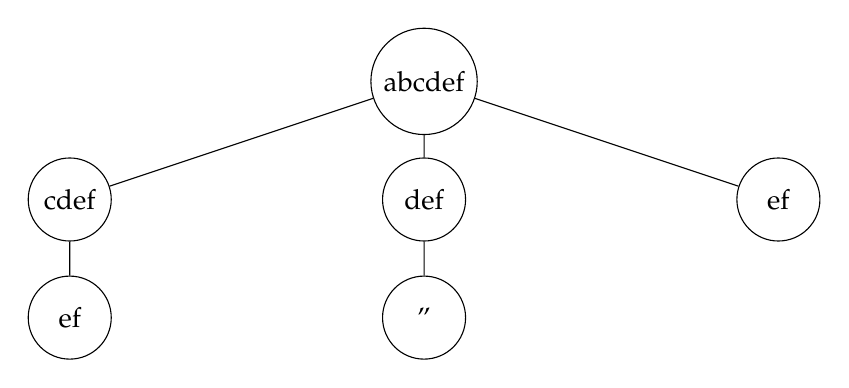
\begin{tikzpicture}[
  every node/.style = {minimum width = 3em, draw, circle},
  level/.style = {sibling distance = 45mm/#1}
  ]
  \node {abcdef}
  child {node {cdef} 
          child {node {ef}}
        }
  child {node {def}
          child {node {''}}
  	   }
  child {node {ef}
 };
\end{tikzpicture}
\end{document}

